% interactcadsample.tex
% v1.03 - April 2017

\documentclass[]{interact}

\usepackage{epstopdf}% To incorporate .eps illustrations using PDFLaTeX, etc.
\usepackage{subfigure}% Support for small, `sub' figures and tables
%\usepackage[nolists,tablesfirst]{endfloat}% To `separate' figures and tables from text if required

\usepackage{natbib}% Citation support using natbib.sty
\bibpunct[, ]{(}{)}{;}{a}{}{,}% Citation support using natbib.sty
\renewcommand\bibfont{\fontsize{10}{12}\selectfont}% Bibliography support using natbib.sty

\theoremstyle{plain}% Theorem-like structures provided by amsthm.sty
\newtheorem{theorem}{Theorem}[section]
\newtheorem{lemma}[theorem]{Lemma}
\newtheorem{corollary}[theorem]{Corollary}
\newtheorem{proposition}[theorem]{Proposition}

\theoremstyle{definition}
\newtheorem{definition}[theorem]{Definition}
\newtheorem{example}[theorem]{Example}

\theoremstyle{remark}
\newtheorem{remark}{Remark}
\newtheorem{notation}{Notation}

\begin{document}
\title{Antisystemic Effects of Antimining Andean Peasant Struggles}

\maketitle

\begin{abstract}
The metabolic structural processes of the capitalist world-economy have produced historical antisystemic resistances with world-scale effects over capital's extended reproduction. The history of the Andean indigenous and cholo peasantry struggles against colonial and imperialist mining constituted a new political identity in absolute contradiction with the dispossession and destruction of land and water as vital values for their social reproduction. While theory has been developed about the antisystemic effects of social movements created by the systemic processes of the world-economy, theorizing on their causal mechanisms is a work in progress, permeable to be developed broadly within a Marxist critique of imperialism political economy. In this article, a causal mechanisms hypothesis is built to explain the world-scale effects of antimining struggles over the finance capital reproduction circuit of mining imperialists bourgeoisies in competition under the gradual breakout conditions of shared imperialism in Los Andes from three case studies: i) the cholo-peasantry antimining struggles in Cajamarca (Peru) during the 2004 and 2011-2012 against the Newmont Gold Mining Corporation headed in the U.S., ii) the indigenous-peasantry mining struggles in Apurímac (Peru) during 2015 and 2019 against the MMG of China Minmetals Corporation (CMC), and iii) the indigenous-cholo peasantry antimining struggles in Cotopaxi (Ecuador) during 2023-2024 against the Atico Mining Corporation headed in Canada. The theory-building case studies conducted have been nurtured by fieldwork, archive research, and protest event data analysis to evidence the consistency of the hypothesis stated on the antisystemic effects of antimining struggles.
\end{abstract}

\begin{keywords}
Peru; Ecuador; China; United States of America; Canada; Antimining struggles; Antisystemic; Capital reproduction; Mining; Imperialism 
\end{keywords}

\begin{abstract}
Los procesos metabólicos de reproducción de la economía-mundo capitalista han producido históricamente resistencias antisistémicas con efectos a escala mundial sobre la reproducción extendida del capital. Las luchas del campesinado cholo-indígena contra la minería colonial e imperialista en Los Andes forman un sujeto político en absoluta contradicción con el despojo y la destrucción de la tierra y el agua como valores vitales para su reproducción social. Si bien se ha desarrollado teoría sobre los efectos antisistémicos de los movimientos sociales creados con los procesos sistémicos de la economía-mundo, la teorización sobre los mecanismos causales que pueden explicar dichos efectos, es una labor en curso permeable a ser desarrollada a la luz de una crítica marxista a la economía política del imperialismo. En este artículo, construyo una hipótesis de mecanismos causales para explicar los efectos antisistémicos de las luchas antimineras sobre la reproducción del capital financiero circulado en la industria minera por burguesías imperialistas en competencia bajo condiciones de ruptura progresiva del imperialismo compartido en Los Andes, a partir de tres estudios de caso: i) las luchas antimineras del campesinado cholo en Cajamarca (Perú) durante los años 2004 y 2011-2012 contra la Newmont Gold Mining Corporation asentada en EE.UU., ii) las luchas del campesinado indígena en Apurímac (Perú) durante 2015 y 2019 contra la MMG de la China Minmetals Corporation (CMC), y iii) las luchas antimineras campesinas cholo-indígenas en Cotopaxi (Ecuador) durante 2023-2024 contra la canadiense Atico Mining Corporation. Los estudios de caso realizados para la construcción de teoría se han nutrido de trabajos de campo, revisión de archivos, así como del análisis de catálogos de eventos de protesta para evidenciar la consistencia de la hipótesis construída sobre los efectos antisistémicos de las luchas antimineras.
\end{abstract}

\begin{keywords}
Perú; Ecuador; China; Estados Unidos; Canadá; luchas anti-mineras; anti-sistémico; reproducción de capital; minería; imperialismo 
\end{keywords}

\section{Introduction}
Los efectos de la resistencia antisistémica del movimiento antiminero en Los Andes expresan el avance del desarrollo de la lucha de clases en la formación identitaria de contendientes históricos en absoluta contradicción (Lenin 1914; Anderson y Hudis 2007) a la reproducción de las burguesías mineras imperialistas que financian el capital a través del circuito minero de acumulación. La minería en Los Andes está en el centro de los procesos fundacionales del sistema-mundo moderno y en los procesos metabólicos de reproducción del capital financiero en la economía-mundo actual. En general, todo el proceso de la vida económica mundial en los tiempos modernos se reduce a la producción de plusvalía y a su distribución entre los diversos grupos y subgrupos de la burguesía sobre la base de una reproducción cada vez más amplia de las relaciones entre dos clases: la clase del proletariado mundial, por una parte, y la burguesía mundial, por otra" (Bukharin, 1929, 1966: 26-27). 

El desarrollo de los procesos de producción y circulación de la minería colonial e imperialista, y de la minería aurífera en particular, han estructurado la formación social y la resistencia histórica del campesinado indígena-choló, contra el militarismo, el despojo y la destrucción expansiva de los valores vitales para su reproducción social: el agua y la tierra. Esto se evidencia con el genocidio de los pueblos "indígenas" de Abya Yala, la explotación de los sobrevivientes en la minería colonial, así como las masacres de sus hijos y nietos proletarizados campesinos indígenas cholos, con la implantación imperialista del capital financiero de los trusts capitalistas monopolistas norteamericanos inter-"nacionalizado" en enclaves mineros de Los Andes. El militarismo como política de expansión de las burguesías imperialistas para controlar o garantizar el funcionamiento del circuito minero para la reproducción de su capital financiero, es un rasgo persistente de la colonialidad de la problemática minera actual. Así como un punto nodal de su solución antiimperialista en Los Andes. 

En el origen de la formación del sistema-mundo moderno que comenzó en el siglo XVI y en el desarrollo de la economía mundial del imperialismo a finales del siglo XIX y principios del XX, las masacres y la explotación del campesinado indígena-cholo proletarizado en las minas de Los Andes operaron como una constante bajo la minería colonial y la minería imperialista. La minería colonial en Los Andes fue el método fundacional de la acumulación original expandida del siglo XVI (Cueva [1977]1999:63-78; Marx [1886]1976:874-875,915) correspondiente a la expansión material de las burguesías bancarias oligárquicas europeas (Arrighi 1994) que emergieron de la concentración del capital mercantil en Oriente Medio durante el siglo XIII (Abu-Lughod 1991), dando forma al sistema-mundo moderno. La minería imperialista es un proceso vital de producción y acaparamiento para la reproducción extendida de capitales financieros con trayectorias diferenciadas de centralización y concentración (Bukharin [1929]1966) que garantizan su inter-"nacionalización" a través del militarismo (Luxemburg [1913]2015). 

En su esfuerzo por conceptualizar los efectos antisistémicos de los movimientos producidos por el proceso estructural sistémico de la economía mundial, Arrighi, Hopkins y Wallerstein (1989:88) trataron los efectos antisistémicos como causados por la centralización del capital como una tendencia a escala mundial altamente desarrollada bajo la economía-mundo del imperialismo y destacaron la divergencia de las [nuevas] ubicaciones sociales potencialmente graves de los movimientos antisistémicos. Sin embargo, aún no se han evidenciado los mecanismos causales que conectan la constitución de identidades antisistémicas en negación absoluta con la necesidad expansiva del metabolismo de la reproducción de capitales financieros en pugna con diferentes niveles de centralización y concentración. A medida que se presentan los acontecimientos, la aparición de nuevos contendientes con distinguidas identidades antagónicas aparece como recordatorio del desarrollo de la historia. 

Son tratados como rastros o más bien pistas para buscar una pregunta de investigación lo suficientemente operativa para una hipótesis de construcción de la teoría del mecanismo causal: ¿Cómo las luchas antimineras tienen efectos antisistémicos sobre la reproducción del capital de las burguesías imperialistas? Sostenemos que los efectos antisistémicos de los retadores históricos formados por los procesos estructurales expansivos vitales para la reproducción de capitales financieros competidores en condiciones de imperialismo compartido en Los Andes, son reales en sus consecuencias. Las luchas antimineras tienen efectos a escala mundial sobre la disminución de la tasa de ganancia: la obstrucción del tiempo de circulación en la transformación de la plusvalía en ganancia, así como la perturbación de la composición orgánica esperada del capital avanzado de las burguesías imperialistas que invierten en el circuito de reproducción minera de acumulación, sobre los trusts del capitalismo de Estado, el acaparamiento monetario de oro y el comercio. 

Los efectos de las luchas antimineras sobre los mecanismos metabólicos de la reproducción del capital son antisistémicos, también porque su identidad antagonista absoluta exacerba la competencia imperialista para la expansión material frente a una próxima repartición de las guerras imperialistas. Planteamos la siguiente hipótesis: las resistencias antisistémicas históricas indígenas-cholas formadas con y en antagonismo con los procesos estructurales sistémicos vitales para la reproducción extendida del capital son reales por sus efectos (Merton 1948). Las luchas antimineras tienen efectos antisistémicos al disminuir la tasa de ganancia esperada de la clase superior de la economía mundial del imperialismo a través del circuito de la acumulación minera, al bloquear efectivamente su circulación de capital mediante actuaciones obstructivas de la lucha. De este modo, retrasando su tiempo de circulación y alterando la composición orgánica esperada del capital financiero, avanzaba en la producción de plusvalía conformada como una masa de capital minero-mercantil, y su posterior metamorfosis en superganancia total. 

Las luchas antimineras de los indígenas cholos, de hecho, desencadenan el acaparamiento de oro por parte de los trusts bancarios estatales imperialistas, porque las tenencias de oro son capital-dinero y capital-mercancía al mismo tiempo. Pero a diferencia del capital monetizado en forma de papel-moneda -moneda pura-, el capital-dinero-oro mantiene su forma de plusvalía de capital-mercancía. Y de esa manera, su transformación en ganancia puede retrasarse cuando la tasa de ganancia disminuye. Como explicaremos aquí en adelante, debido a la demora en la circulación del capital financiero de los trusts estatales de los capitalistas bancarios internacionales, la obstrucción antisistémica de las luchas antimineras desencadena el aumento de la magnitud constante del capital de su composición orgánica de capital, amplificando su efecto decreciente en la tasa de ganancia, y en consecuencia una cantidad reducida de plusvalía se transforma en ganancia total. En efecto, perturbando la producción de plusvalía y la tasa de ganancia esperada por las burguesías imperialistas en la continua competencia militarista por la expansión de sus circuitos de acumulación minera, mediante guerras imperialistas o intervenciones imperialistas orientadas a establecer sus relaciones de producción en las "economías-nacionales" en las que se encuentran las materias primas preciosas de la minería, como en Los Andes.

\section{Resistencia antisistémica de los impugnadores históricos: el movimiento antiminero del campesinado indígena-cholo andino}

La formación de la estructura de clases del sistema-mundo moderno se basa en la división internacional racializada del trabajo producida por la colonización como política de expansión del capital mercantil. Alrededor de diez millones de "indígenas" sobrevivieron al genocidio planeado en Los Andes de un total estimado de sesenta y cinco millones exterminados en la "América" continental, siendo sublimados como seres inferiores y reducidos a mera fuerza de trabajo por el método de colonización de la acumulación primitiva (Marx [1886]1976:873-875, 914; Mariátegui, 16 de enero de 1929:78; Quijano y Wallerstein 1992; Quijano [1999], 2007, 169-170; Mignolo 2011, 183-84). El mundo ya no cabía en la conciencia de los supervivientes. Pero en su conciencia colectiva sobrevivió un mito. O un mito tiene sentido en nuestra conciencia, es el mito del nuevo indígena, del Inkarri (el retorno Inka), del Yawar-Inti (Sol de Sangre) y el resurgimiento del mundo "indígena" por una venganza revolucionaria. En oposición a la interpretación de Arboleda (2020) de la formación de la "política de identidad" indígena (Martín Arboleda afirmó: "Ya en la década de 1990, antes de que las llamadas "políticas de identidad" ganaran protagonismo en los círculos académicos internacionales, el filósofo ecuatoriano Bolívar Echeverría —un reconocido teórico del sincretismo cultural y la modernidad capitalista en América Latina— ya estaba desconcertado por los esencialismos culturales autodestructivos de las variantes emergentes de los indígenas latinoamericanos política. 

Las culturas prehispánicas en las Américas, argumentó, estaban apuntaladas por cosmologías profundamente relacionales y, por lo tanto, eran incapaces de percibir al "Otro" como una alteridad independiente. La otredad que percibían en los colonizadores españoles era para ellos una mera variante de la mismidad de su propio yo colectivo. La mentalidad europea, en cambio, siempre interpretó al otro cultural en términos de alteridad radical, como negación absoluta de su propia identidad" (Arboleda 2020:210).}, sostengo que la subjetividad revolucionaria que conjura el socialismo indígena es una formación histórica en movimiento, un bloque de texto histórico vivo que choca, desarrollando al campesinado como una clase antagonista en subsunción formal desde el siglo XVI. Tanto para Arboleda (2020) como para Bolívar Echevarría, los pueblos indígenas no podían entender el antagonismo entre ellos y los españoles. Su cosmología, creen, no permitió que los indígenas se dieran cuenta de que estaban siendo asesinados por un colectivo externo antagónico a sus vidas o a su "yo colectivo". Si alguien sigue ese argumento, por implicación, estos "esencialismos culturales autodestructivos" autóctonos sólo cambiarían con la posterior apropiación de la lógica hegeliana como base para la reproducción de la racionalidad sublimadora de la "mentalidad europea". Es decir, desde el encuentro de los pueblos "indígenas" con esta "mentalidad europea", sus descendientes son capaces de interpretar "al otro cultural en términos de alteridad radical, como una negación absoluta de su propia identidad". 

En suma, hay que entender que Bolívar Echevarría debió omitir ideológicamente la obra del antropólogo peruano Luis E. Valcárcel, para no forzar una aproximación a la obra de José Carlos Mariátegui, quien encontró un sujeto revolucionario indígena ya en marcha cuando iban a trabajar en su politización a principios del siglo XX. Afortunadamente, el trabajo de Alberto Flores Galindo ([1985]2010) hizo justicia a esta problemática al rastrear el mito de los Inkarri en luchas indígenas y populares emblemáticas de la historia del Perú. A medida que los primeros intelectuales obreros se convirtieron en los profetas de este mito, el socialismo indígena se forjó a principios del siglo XX como la convergencia del "grupo cholo" El "grupo cholo" es un estrato social cuya formación surge de la masa del campesinado indígena servil o semiservil, diferenciado por la incorporación de elementos de la cultura criolla occidental. Sin embargo, al mismo tiempo, sostienen, preservan y reconocen su diferencia y sus orígenes en la cultura indígena y en la estructura social del campesinado indígena, como la formación social de la que partimos (Quijano 1980: 63-65).} con el campesinado indígena en resistencia histórica. 

El trabajo de politización socialista emprendido por Mariátegui, Mayer y Valcárcel (entre otros) en la organización de las bases del socialismo en el Perú y en la creación del socialismo indígena, encontraron ya en marcha el mito del resurgimiento indígena. En cuyo marco de interpretación, la revolución se lleva a cabo como venganza por los nuevos indígenas, sus remanentes, sus hijos y nietos. La revolución socialista como movimiento y horizonte ya operaba en Los Andes, cuando El Amauta José Carlos Mariátegui y el grupo cholo que constituyó con otros intelectuales trabajadores del proletariado en formación, iniciaron su labor de politización. Mariátegui escribió en el prólogo de La tempestad de Valcárcel en Los Andes (1927): "Recuerdo el inesperado e impresionante tipo de agitador que encontré hace cuatro años en el indígena de Puno Ezequiel Urviola. Este encuentro fue la mayor sorpresa que el Perú tenía reservada para mí a mi regreso de Europa. Urviola representaba la primera chispa de un fuego que estaba por llegar. Era el indígena revolucionario, el indígena socialista. Tuberculoso, jorobado, sucumbió después de dos años de trabajo incansable. Hoy no importa que Urviola no exista. Basta con que existiera. Como dice Valcárcel, hoy las montañas están preñadas de Espartaco" (Mariátegui en el prólogo a Valcárcel 1927:11). 

La historia de la lucha de clases en Los Andes definitivamente precede al socialismo, pero lo más importante es que el campesinado indígena-cholo aprendió a instrumentalizarlo. Así, para el primer cuarto del siglo XXI, el campesinado indígena-cholo no solo ha instrumentalizado efectivamente el socialismo (y el marxismo) sino también el ambientalismo (Mejía 2021; 2024), fijando su articulación discursiva en el reconocimiento de entidades sensibles como montañas, ríos y lagunas (de la Cadena 2010). Como enfatizó De la Cadena sobre la obra visionaria de José María Arguedas: "[l]a totalidad, Todas las Sangres propuso un movimiento social indígena alternativo, aliado crítico de la izquierda moderna, pero con una lógica híbrida a-moderna propia. La alfabetización y la política moderna eran importantes, pero tenían que ser utilizadas y traducidas selectivamente, en lugar de erradicar las costumbres indígenas" (2005:18). La hibridez en este sentido es performativa y no una reproducción de la modernización occidental como aculturación, sino que los cholos como descendientes indígenas han ido construyendo su propia lógica cultural que reconoce sus orígenes, a la vez que se apropian de objetos culturales occidentales-modernos, como hacemos con los marcos de interpretación socialistas y ecológicos en las luchas mineras y mineras del siglo XXI. Como evidencia se destacan los tres estudios de caso: i) las luchas antimineras cholo-campesinas en Cajamarca (Perú) durante los años 2004 y 2011-2012 contra la Newmont Gold Mining Corporation encabezada en EE.UU., ii) las luchas mineras indígenas-campesinas en Apurímac (Perú) durante 2015 y 2019 contra la MMG de China Minmetals Corporation (CMC), y iii) las luchas antimineras indígenas-campesinas cholo en Cotopaxi (Ecuador) durante 2023-2024 contra Atico Mining Corporation encabezada en Canadá. El campesinado cholo-indígena actualizó su interpretación de la minería desde una perspectiva de clase, nutrida por los discursos ecológicos y la cosmopolítica indígena (de la Cadena 2020) en defensa del agua, la tierra, la vida y la biodiversidad.

\subsection{La resistencia histórica de las luchas campesinas cholo-indígenas contra la minería imperialista en Los Andes}

La minería imperialista es un proceso productivo y de acaparamiento central para la reproducción extendida del capital de los trusts de los capitalistas de Estado bancarios... "El desarrollo de las sociedades anónimas, que permitió utilizar el capital de un número considerable de empresarios individuales, y que socavó radicalmente el principio de la propiedad individual de las empresas, creó las condiciones previas para las grandes asociaciones monopolistas de empresarios. La concentración del capital asumió aquí una nueva forma, a saber, la forma de concentración en trusts. La acumulación de capital ya no aumentaba el capital de los productores individuales; Se convirtió en un medio para aumentar el capital de las organizaciones de empresarios. [...] Las ramas individuales de la producción están entretejidas de diversas maneras en un cuerpo colectivo, organizado en gran escala. El capital financiero se apodera de todo el país con mano de hierro. La "economía nacional" se convierte en un gigantesco fideicomiso combinado cuyos socios son los grupos financieros [bancos] y el Estado. A estas formaciones las llamamos trusts capitalistas de Estado" (Bukharin [1915]1988:117-118).}, como las formaciones económicas más avanzadas de la economía mundial... "La economía del mundo incluye todos estos fenómenos económicos que, en general, se basan en las relaciones entre los seres humanos comprometidos en el proceso de producción. En general, todo el proceso de la vida económica mundial en los tiempos modernos se reduce a la producción de plusvalía y a su distribución entre los diversos grupos y subgrupos de la burguesía sobre la base de una reproducción cada vez más amplia de las relaciones entre dos clases: la clase del proletariado mundial, por una parte, y la burguesía mundial, por otra" (Bukharin, 1915, 1988: 26-27). del imperialismo en competencia por su inter-"nacionalización".\nota {Este concepto se explica ampliamente en la siguiente sección.} 

Aunque las bases institucionales y militares de la dominación imperialista en Los Andes se asentaron con la implantación del capital financiero monopólico de los trusts capitalistas más centralizados de los EE.UU., a través de enclaves extractivos para las industrias más rentables en las "nacionales" semifeudales y semicoloniales durante el período de 1895 a 1930. Desde principios del siglo XX, la industria minera de Los Andes estuvo bajo el control casi exclusivo de la burguesía imperialista estadounidense. La minería fue una de las industrias donde el capitalismo se desarrolló más rápidamente, especialmente en Los Andes, donde a partir de 1895 el capital monopolista se dirigió hacia la minería a gran escala, la producción de petróleo y la agricultura (Mariátegui [1928]2011:245-249; Cueva [1977]1999:63-64; Quijano [1977]1988:114-121). De hecho, las luchas de los sindicatos mineros del altiplano central peruano estuvieron ejecutando una activa resistencia antisistémica desde su génesis con la primera huelga minera contra la Corporación Cerro de Pasco (CPC) del 7 de enero de 1919 -inspirada en los avances del proletariado en Europa y la Revolución Soviética de octubre de 1917 (Melgar Bao, 2020:132)- hasta finales de la década de 1980. Los procesos de formación sindical y politización del proletariado minero del altiplano central del Perú atravesaron una trayectoria de radicalización durante la mayor parte del siglo XX. Esta trayectoria de radicalización se extendió a las minas medianas y pequeñas a nivel nacional, así como a las minas del altiplano sur –como lo evidenciaron las masacres de 1957 y 1966 en las minas de Toquepala (Moquegua), explotadas por la Southern Peru Copper Corporation (SPC)–. Las minas se abrieron para la "nacionalización" del capital financiero de la burguesía imperialista estadounidense a través del contrato Cuajone, firmado secretamente por el gobierno militar "nacionalista" de Velasco Alvarado. La Southern Peru Copper Corporation (SPC) fue fundada en 1952 por la American Mining and Smelting Company (ASARCO), que en la primera década de 1900 operaba el circuito de reproducción minera de los portadores de capital financiero. como la Phelps Dodge Overseas Capital Company, la Cerro de Pasco Corporation (CPC) y la Newmont Mining Company, que ya concentraban hacia 1901 el 20 por ciento de la fundición de cobre y el 15 por ciento de la refinación del cobre a escala mundial (Pérez-Jiménez, 2020:25). 

Evidenciando la continuidad de la operación monopólica exclusiva de las burguesías imperialistas norteamericanas, las formaciones centralizadas en el Perú durante todo el siglo XX.} Mientras que durante la década de 1980 se consolidó la cooptación de los sindicatos de trabajadores mineros de la Corporación del Cobre del Sur del Perú (SPC) como resultado de la aplicación de su trayectoria de institucionalización. Por su parte, la intensidad y dureza del militarismo ejecutado contra las protestas de los mineros en el altiplano central peruano explotado por la Corporación del Cobre Cerro de Pasco (CPC), evidenció la irrupción de la transgresión llevada a cabo por las luchas mineras como desafío directo al principal circuito de reproducción de la acumulación de capital. La aplicación sistemática del militarismo es la única garantía para sostener su política imperialista sobre las minas del altiplano central del Perú se evidenció en las masacres de Malpaso (1930), Cobriza (1971), así como en la represión militarizada de la campaña de paro minero de mediados de los 80 reprimida con el encarcelamiento de cientos de mineros sindicalizados, y el asesinato de Saúl Cantoral en 1988 por el grupo de tareas "Comando Rodrigo Franco" (una organización criminal paramilitar de aniquilación que operó bajo el primer gobierno de Alan García). 

Sin embargo, la radicalización de las huelgas mineras se desarrolló frente a la represión militarizada y los regímenes militares. La formación de una vanguardia del proletariado peruano en abierta confrontación con la burguesía minera imperialista estadounidense, se desarrolló hasta la década de 1980, cuando el Partido Comunista del Perú-Sendero Luminoso (PCP-SL) y el Movimiento Revolucionario Túpac Amaru (MRTA) iniciaron las luchas armadas. La trayectoria de radicalización de las luchas de los mineros se convirtió en un desafío antiimperialista, operado en un contexto caracterizado por la escalada de la lucha armada en América Latina, por las consecuencias de la secesión chino-soviética y la resolución de las guerras imperialistas entre la U.R.S.S. y los EE.UU. La formación de la base para la centralización horizontal del capital financiero chino-estadounidense se desarrolló, gradualmente después de la resolución imperialista compartida de la guerra de Vietnam, y la posterior implementación de reformas de mercado en China por Deng XiaoPing en 1978, hasta los primeros años del siglo XXI, marcados por los ataques del 11 de septiembre de 2001 en Wall Street. el Pentágono y la Casa Blanca. Cuando, en condiciones de imperialismo compartido, estos capitales financieros inician un proceso de separación y ruptura, reduciendo paulatinamente su centralización horizontal. Por lo tanto, se restringe la "nacionalización" de los capitales bancarios estadounidenses como capital financiero que circula a través de las formaciones económicas de la producción industrial de China. De hecho, las burguesías imperialistas de Estados Unidos y China comparten las condiciones de acumulación para su mutuamente consentida concentración de capital e inter-"nacionalización" en el período comprendido entre los años 70 y la primera década de los 2000, con un punto de quiebre en los años 2013-2015, que denota un desenredo inicial de sus tasas de ganancia, que podría extenderse levemente hasta 2019. con una reciente afirmación entre 2021 y 2023, que se supone reforzada con los datos actualizados que consideran la contienda interestatal de 2024. Considerando su estimación como un indicador del monto de capital monetizado responsable del intercambio de reservas de oro-dinero-capital como un fondo de reserva de plusvalía congelada bajo la forma de oro-mercancía-capital y oro-dinero-capital al mismo tiempo (Figura 4). 

El capital financiero avanzó en la "nacionalización" de una China altamente centralizada en la que los capitalistas de estado confiaban durante la década de 2000, y gradualmente aprovechó las condiciones institucionales y militares establecidas por las burguesías imperialistas estadounidenses para operar en el Perú. En veinte años, el capital financiero fiduciario de los capitalistas estatales de China construyó una expansión considerable de su participación en la minería del cobre peruana, aunque todavía incipiente en la minería del oro, a través de la Corporación de Minmetales de China (CMC). Las burguesías mineras imperialistas diferenciadas están en el núcleo de la organización inter-"nacionalizada" del capital financiero, subyugando la producción minera industrial de las "economías-nacionales" semicoloniales en Los Andes a todo el circuito de reproducción de las formaciones económicas más elevadas resultantes de trayectorias diferenciadas de centralización a escala de "economía nacional". Correspondiente a los niveles más altos de concentración de capital de la economía-mundo del imperialismo, desde la transición de Gran Bretaña a la hegemonía del sistema-mundo moderno de los EE.UU., alrededor de los primeros años del "largo siglo XX" (Arrighi 1994). 

Bajo esta coyuntura de ruptura del imperialismo compartido en Los Andes, se instrumentaliza indiscretamente un régimen político de militarismo y violencia estatal terrorista para garantizar la máxima tasa de plusvalía y tasa de ganancia para las formaciones económicas de capa superior a escala mundial. Sin embargo, la descentralización horizontal del capital financiero chino-estadounidense tiene efectos diferenciados para el circuito de acumulación de cada burguesía imperialista, de acuerdo con sus propios niveles de concentración y centralización. Además, los efectos a escala mundial de la avanzada descentralización horizontal de los capitales financieros chino-americanos, exhiben consecuencias diferenciadas sobre los procesos estructurales sistémicos de producción y circulación, configurando la próxima formación transitoria que necesariamente implicará una nueva división internacional del trabajo.

\section{La hipótesis de los efectos antisistémicos para las luchas antimineras}

El avance del capital-dinero por parte de los capitalistas bancarios a través del circuito de reproducción minera en Los Andes produce plusvalía moldeada y ponderada como capital-mercancía, lista para ser convertida en la forma de ganancia total de plusvalía por su venta en el mercado, en cuyo caso su forma de plusvalía ha desaparecido. Pero, en el caso del oro, al mismo tiempo puede ser considerado como capital dinerario capaz de ser transformado en ganancia por su cambio por capital monetario en moneda pura, o puede ser oro acumulado bajo su forma de capital mercantil. De ahí que, además de la aterradora ilustración de este "personaje fundamental", el bello dualismo teórico. En la medida en que examina el capital en su capacidad profesional, la economía ilustrada desprecia el oro y la plata con el mayor desdén, como si fueran la forma más indiferente e inútil de capital. Sin embargo, desde el momento en que se trata de la banca, este aspecto de las cosas se invierte y se convierte en el capital por excelencia, para cuya conservación hay que sacrificar todas las demás formas de capital y trabajo. Pero, ¿de qué manera se distinguen el oro y la plata de otras formas de riqueza? No por la magnitud del valor, pues éste está determinado por la cantidad de trabajo materializado en ellos. Sino más bien como encarnaciones y expresiones autónomas del carácter social de la riqueza. La existencia social que tiene aparece como algo más allá, como una cosa, objeto o mercancía fuera y al lado de los elementos reales de la riqueza social. El crédito, al ser una forma social de riqueza, desplaza al dinero y usurpa su posición. Es la confianza en el carácter social de la producción lo que hace que la forma dinero de los productos aparezca como algo meramente evanescente e ideal, como una mera noción. Pero tan pronto como el crédito se tambalea, y esta es una fase necesaria en el ciclo de la industria moderna, se supone que toda la riqueza real se transforma realmente en dinero, en oro y plata, una demanda descabellada, pero que necesariamente surge del sistema mismo. Y el oro y la plata que se supone satisfacen estas inmensas reclamaciones ascienden en total a unos pocos millones en las bóvedas del banco. Por lo tanto, un drenaje de lingotes muestra de la manera más notable por sus efectos que la producción no está realmente sujeta al control social, como proceso social, y que la forma social de la riqueza existe junto a la riqueza misma como cosa. El sistema burgués tiene esto en común con los sistemas anteriores en la medida en que se basan en el comercio de mercancías y el intercambio privado. Pero sólo con este sistema surge la forma más llamativa y grotesca de esta absurda contradicción y paradoja, porque: 1) en este sistema la producción para el valor de uso directo, para el uso propio del productor, está completamente abolida, de modo que la riqueza sólo existe como un proceso social que se expresa en el entrelazamiento de la producción y la circulación; y (2) con el desarrollo del sistema crediticio, el sistema burgués se esfuerza constantemente por abolir esta barrera metálica, que es tanto una barrera material como una barrera imaginaria para la riqueza y su movimiento, mientras que una y otra vez se golpea la cabeza contra ella" (Marx, [1984-1865]2017: 671-672).} (ver Figura 2 y Figura 3). 

De esta manera, el oro conserva su forma de plusvalía incorporada en el volumen de capital-mercancía aurífera producido por una determinada composición orgánica de capital financiero adelantado para la minería en condiciones naturales, culturales e históricas concretas. Las condiciones naturales y culturales son determinantes para la reproducción del capital financiero invertido en la producción minera y comercialización por los trusts de los capitalistas de Estado bancarios. Cuando las formaciones económicas se desarrollaron con los procesos de concentración y centralización y saturaron su escala de "economía nacional", la feroz competencia por un desarrollo de inter-"nacionalización" altamente avanzado operó por el militarismo puro de las guerras imperialistas en Ucrania, Palestina y probablemente pronto en Taiwán. 

Y por medio de intervenciones de securitización imperialistas sobre "nacionales-economías" semicoloniales, como la represión militarizada por los levantamientos masivos de Ecuador (2019) (Iza, Tapia y Madrid 2020), Chile (2019), Colombia (2020-2022), Perú (2022-2023) (Montoya y Quiroz 2023), y más recientemente Venezuela (2024). Por "internacionalización" entendemos el proceso en el que los trusts de los capitalistas bancarios organizan la asignación de su capital-dinero lanzado como "inversión extranjera directa" a las industrias más rentables y estratégicas, convirtiéndose en capital financiero situado en el territorio de un Estado semicolonial con el fin de su reproducción. Aprovechando las diferencias salariales correspondientes a la división mundial del trabajo ocultas bajo el fenómeno menos misterioso y antiguo de la "globalización", la "transnacionalización" o la muy honesta "internacionalización" de la producción en la economía-mundo del imperialismo (Marx [1864-1865]2017:47-54; Bukharin [1915]1966:17-18, 53, 60-62; Lenin [1917]1964:260, 265-266, 278-279). 

La función del fondo de reserva, la reserva de lingotes del Banco, una función que no es el único determinante de su formación, ya que el fondo puede crecer simplemente por el hecho de que el comercio exterior e interno está paralizado, es triple: (i) es un fondo de reserva para pagos internacionales, de hecho, un fondo de reserva de dinero mundial; (ii) es un fondo de reserva para la circulación de monedas nacionales, que se expande y se contrae; y (iii) (y esto está relacionado con la función bancaria y no tiene nada que ver con la función del dinero simplemente como dinero) es un fondo de reserva para el pago de depósitos y la convertibilidad de los pagarés" (Marx [1864-1865]2017:667)} proporcional a una cantidad potencial esperada de capital-dinero que son capaces de realizar mediante el proceso de circulación en la transformación de la plusvalía en ganancia (Marx, [30 de abril de 1868]1988:21-24). Garantizando sus escalas de reproducción diferenciadas para una etapa posterior del desarrollo del capitalismo, en un momento histórico en el que la tendencia irresoluta de sus contradicciones se expresa en la crisis del imperialismo ecológico, productivo y compartido. Las luchas antimineras tienen efectos antisistémicos, obstruyendo el circuito de reproducción minera de ciertos capitales financieros. Más específicamente, las exitosas campañas contenciosas de protestas mineras y luchas antimineras en Los Andes involucraron la ejecución sostenida de performances obstructivas (por ejemplo, la huelga) que una categoría de actores políticos (por ejemplo, los trabajadores mineros) aprende a exigir la reivindicación de las demandas colectivas, frente a un determinado contendiente (por ejemplo, empresas mineras privadas y estatales) (Tilly y Tarrow 2015:14).} de lucha, como el bloqueo de carreteras o la ocupación protectora de montañas y lagunas, como se ha hecho en Cajamarca y Apurímac en Perú, y Cotopaxi en Ecuador, como en otros territorios de Colombia, Chile y más recientemente Argentina, para frenar los proyectos mineros imperialistas (Mejía 2021:97-99). 

En efecto, el campesinado indígena-cholo bloquea la producción y el transporte de un volumen comprometido de capital-mercancía minera, durante un tiempo de circulación esperado y con una composición orgánica predeterminada. El aumento del tiempo de circulación en la transformación de la plusvalía en ganancia, retrasa el consumo del capital financiero invertido en capital constante, aumentando la diferencia entre la tasa de plusvalía y la tasa de ganancia, transformando de hecho una magnitud reducida de la plusvalía en ganancia total. When the surplus value is transformed into total profit during an expected circulation time, i.e. a year, the following dynamics describe this process of metamorphosis, 
\(s'\)\xrightarrow{meta}\(p'\) (Marx [1864-1865]2017:49-55):

(i) The total capital advanced (\textit{C}) to any circuit of reproduction have two components: constant capital (\textit{c}), and variable capital (\textit{v}). As \textit{v} is always necessarily greater than cero, if \textit{c} is  greater than cero, then \textit{C} is greater than \textit{v}.
\[\(C=v+c\);\((v>0\land\(c\)\geq\)0\))\implies{C>v}\)\]
(ii) The rate of surplus-value \textit{(s')} is equal to the ratio of the surplus-value \textit{(s)} and the variable capital \textit{(v)}; and the rate of profit \textit{(p')} is equal to the ratio of the surplus-value \textit{(s')} to the total capital \textit{(k)}: 
\[\((s'=s/v)\land\((p'=s/C)\implies{s'>p'}\]
(iii) The difference between the rate of surplus-value \textit{(s')} and the rate of profit \textit{(p')} is related to the rate of profit \textit{(p')} as the constant capital \textit{(c)} is related to the variable capital \textit{(v)}. And, the rate of profit \textit{(p')} is related to the rate of surplus-value \textit{(s')}as the variable capital \textit{(v)} is related to the total capital \textit{(C)}:
\[[(s'-p')/p')|c/v]
\land\  [(p'/s')|v/C]\]
(iv) The more the constant capital \textit{(c)} increases, the more the difference between the total capital \textit{(C)} and the variable capital \textit{(v)} grows, and the smaller the proportion expressed by the rate of profit\textit{ (p'=s/C)} in comparison with the rate of surplus-value \textit{(s'=s/v)}, or the proportion yield as rate of profit from the rate of surplus-value\textit{ (p'/s')} that is related to the excess of the rate of profit \textit{(s'-p')}:

if (i): \forall \ C:v>0\land\(c\) \geq\) 0\)\
\[\mathcal\vartriangle{(C-v)}\dependent\triangledown(p'/s')\mid\vartriangle\(c\)

if (ii): \exists \ C:\(c>0\) \implies{\((s/v > s/C)\) \iff \exists \ C:\(c=0\)\implies{C =v}

\[\mathcal\vartriangle{c}\dependent\vartriangle\((s'-p')\)\implies({\mathcal\vartriangle{c}\mid\mathcal\triangledown{v})}\dependent\triangledown{\(C\)}\)\

As a whole, the reproduction of finance capital \textit{(M-C-M')} implies the transformation of money-capital \textit{(M)} into productive-capital \textit{(P)}, \textit{\(M-C-M' \implies{ M-P-C-M'}\)}, for an expected higher rate of profit \textit{(p')} equal to the ratio between the surplus-value \textit{(s)} already frozen in certain volume of commodity-capital \textit{(C)} --a super-profit produced by the selected super-exploitation of  higher productive unpaid concrete work-time-life due to the lower wages paid in comparison of the magnitude of variable capital \textit{(v)}that would be invested in the “national-economies" where the realization of the surplus-value \textit{(s)} exploited is converted into augmented money \textit{(M')} as profit--, and the total capital advanced \textit{(C)} (Marx, [30 April 1868]1988:21-24; Bukharin, [1915]1966:81-83).

The circuit of mining capital accumulation of the imperialist bourgeoisies cannot achieve the transformation of their finance capital into increased money-capital, as total profit, because of the operation of the following mechanisms over the dynamics of the metamorphosis process by which the surplus-value takes its profit form (see above): 

1) delaying the circulation of the surplus-value transformation into total profit, and 

2) disrupting the expected organic composition of finance capital  advanced in the production of surplus-value, and in its posterior transformation into total profit; which 

3) trigger the gold hoarding by imperialists bank state trusts, because gold-holdings are money-capital and commodity-capital at the same time, but in contrast with monetized-capital in form of paper ("monopoly") money -pure currency-, gold-money-capital can hold its surplus-value form of commodity-capital, in that manner delaying its transformation in profit when the rate of profit decreases;  

4) as we just explained above, the increment of the constant capital magnitude decreases the rate of profit, as a reduced amount of surplus-value is transformed into total profit, as a result of the delay in the circulation of the finance capital due to the antisystemic obstruction of anti-mining struggles; 

5) indeed, disrupting the rate of surplus value and rate of profit of the imperialists bourgeoisies in ongoing militarist expansion of their mining accumulation circuits by mean of imperialist wars or imperialists interventions oriented to establish its relations of production in the “national-economies" at which the mining precious “raw" materials are situated.

In this sense, the indigenous-cholo peasantry antimining struggles challenge the circulation of the finance capital of the imperialists mining bourgeoisies, obstructing the production and circulation of mining commodities. The circuit of mining capital accumulation obstruction reduce the amount of surplus-value able for its realization as profit, reached by the sell of the mineral raw materials shaped as a volume of commodity-capital. If the time of circulation and organic finance capital composition are disrupted, the expected rate of super-profit decreases, and the gold-money-commodity-capital appears as the preferred shape of capital to hold its surplus-value form, until the rate of super-profit increases enough to finish its circulation process as pure monetized total profit.

En este punto puede sostenerse un argumento psicológico, si no sustancial. La racionalidad económica, tal como es contextual, espera una oportunidad, un signo de fortuna que potencie su virtud. La ventana de oportunidad debe tener el tamaño correspondiente a la satisfacción de su expectativa ideológica sobre cuánto ellos (los capitalistas de capa superior sindicados en los trusts de capitalistas de estado de bancos internacionales que poseen el capital mundial de oro) pueden aumentar su diferenciación de clase por el tipo de oportunidad para la reproducción del capital que puede satisfacer su voluntad de poder como la metamorfosis de convertirse en algo diferenciado. sublimados, alienados por la explotación y dominación de los demás como condición media y necesaria-suficiente de su existencia en la formación económica que constituyen como una clase imperialista mundial integrada por los capitalistas sindicados en los trusts capitalistas de los Estados bancarios internacionales. Este medio se diferenció, se alienó, se sublimó, obviamente no (sólo) de sus clases antagónicas mundiales (como la historia no se repite, no es un proceso de acumulación primitivo de despojo a escala mundial). Eso ya estaba concedido a escala mundial, ya que la división inter-"nacional" del trabajo de la economía-mundial estaba completando o saturando sus relaciones de producción, al tiempo que desarrollaba sus procesos de concentración y centralización inter-"nacionalmente". De los cuales son parte la descentralización horizontal de las formaciones económicas chino-americanas y sus relaciones de producción y circulación, bajo condiciones de ruptura del imperialismo compartido. Así como las guerras imperialistas y las intervenciones militares por las que la contienda geopolítica y geoeconómica desarrolla su competencia. El proceso de diferenciación de clases es un resultado intencionado de la guerra económica y política en la que se enfrentan los miembros de la capa superior de los bancos internacionales de confianza de los Estados-Estados. El proceso de diferenciación no está impulsado por la producción de plusvalía en forma de capital-mercancía, sino por la circulación de fondos de capital mundial sobreacumulados como capital-dinero-financiero en un proceso de reproducción por una tasa o ganancia más alta. Se espera que la acumulación resultante de capital mundial aumentado alcance un punto crítico cuantitativo en el que se logre un cambio cualitativo de los efectos a escala mundial en el proceso de concentración de capital que implicó la preparación de la más cruda de las guerras imperialistas. De esa manera se destruye el avance de las fuerzas competitivas y de las viejas fuerzas productivas, y se pueden implantar las nuevas relaciones de producción para organizar una economía-mundo para la reproducción del capital-mundo de esta capa superior de capitalistas sindicados en los trusts de capitalistas de estado del banco internacional que gobiernan la contienda geopolítica y geoeconómica. Con consecuencias no solo sobre la estructura de clases y los modos de producción de la economía mundial, sino principalmente sobre las condiciones naturales, culturales e históricas de nuestra reproducción social. En su psicología atomizada, se espera que una mayor cantidad de capital adelantado como capital financiero en "economías nacionales" productivas más altas resulte en una tasa de ganancia más alta. De hecho, el acaparamiento de oro opera como un fondo de reserva que expresa la contradicción entre la acumulación de capital monetario monetizado y el capital oro-dinero en las reservas nacionales de EE.UU. y China, en particular. Parece como si el trust estatal de los capitalistas bancarios de EE.UU. se estuviera preparando para la transformación de un cierto volumen de capital-oro-dinero en capital monetizado soportado en proporción inversa por el trust-trust estatal capitalista bancario de China. Y viceversa. Su voluntad de sublimación, su voluntad de poder, impulsa su voracidad competitiva en una fiebre del oro. Atesorados el fondo de oro, esperan una oportunidad para terminar su circulación como capital-dinero. La reproducción de un inmenso volumen de capital monetizado (acumulado en forma de moneda hegemónica en dólares estadounidenses) en las condiciones existentes imposibles de invertir productivamente en la reproducción de su capital. A partir de ese momento, una parte de su ganancia total, correspondiente a la ganancia de la empresa, circulará como capital avanzado (financiero) en la siguiente etapa de la producción minera, otra parte se pagará como renta, otra se acumulará por intereses-beneficio. La parte de la ganancia de la empresa que es imposible invertir como capital adelantado, se acumula en exceso como un fondo de reserva de capital monetario del cual una porción minúscula puede ser gastada por los capitalistas de la capa superior que la poseen. Por su parte, las condiciones históricas expresadas en las luchas antimineras indígena-cholas de Los Andes en pugna directa con las formaciones económicas más avanzadas del imperialismo-economía mundial, evidencian también un avanzado desarrollo del proceso histórico de la lucha de clases. Las luchas antimineras tienen efectos a escala mundial en la disminución de la tasa de ganancia debido a la obstrucción del tiempo de circulación, en la transformación de la plusvalía en ganancia, además de perturbar la composición orgánica del capital adelantado por el circuito minero de reproducción, en el acaparamiento monetario de oro por parte de los trusts estatales de los capitalistas bancarios. Tienen un efecto antisistémico en el circuito de acumulación extendida de capital de las burguesías imperialistas al bloquear la expansión de su frontera minera extractiva y obstruir la producción y el comercio de minerales en general, y de oro en particular.

\section{Antimining struggles blocking the expansion of the U.S. gold mining extractive frontier in Cajamarca}

La expansión de la frontera extractiva de Minera Yanacocha-Newmont en Cajamarca ha sido impugnada por un movimiento minero que emplea lo que se llama una estrategia de frente única. Ha demostrado ser eficaz en la creación de suficiente poder social popular para enfrentar la minería imperialista. La dureza de la represión militar contra el movimiento minero popular y principalmente campesino en Cajamarca reveló la crueldad de la dominación imperialista en el Perú, justo después de la elección democrática de un presidente de origen nacionalista y militar (Ollanta Humala). Las luchas mineras en Cajamarca nos enseñaron que las luchas campesinas pueden ser interpretadas y desarrolladas como luchas antiimperialistas, ya que implican un enfrentamiento de clases entre dos extremos de la acumulación capitalista: la burguesía minera internacional y el campesinado indígena. El desafío que representan las luchas mineras para el núcleo central de la dominación imperialista en países donde la minería constituye el principal enclave de la acumulación capitalista, apunta al carácter estratégico de las luchas mineras. Son la punta de lanza para el desarrollo de un movimiento antisistémico, así como críticos para las necesidades geoeconómicas de la dinámica de la acumulación de capital durante la actual crisis sistémica (Veltmeyer 2015:124; Wallerstein 2002:38). Las luchas mineras por la defensa de la montaña Quilish y las fuentes de agua de Cajamarca en 2004 han demostrado la efectividad de la estrategia de frente único: se han sumado a los esfuerzos de múltiples organizaciones. Entre ellas se encuentran: las rondas campesinas, las juntas de riego, las rondas urbanas, el sindicato de maestros a nivel provincial y distrital (SUTEP-Cajamarca), fracciones del PCP-PR de Cajamarca, estudiantes universitarios y ONG ambientalistas como Ecovida y Grufides. Desde el inicio de la lucha contra el proyecto minero Conga de Minera Yanacocha-Newmont en noviembre de 2011, los frentes de defensa del medio ambiente se enfrentaron al gobierno del recién electo presidente Ollanta Humala, quien había prometido a los campesinos que las lagunas de Cajamarca no serían destruidas ni se permitiría la minería sin el consentimiento popular. En este contexto, la sostenida campaña minera contra el proyecto Conga de Minera Yanacocha-Newmont se intensificó, impugnando no solo a la empresa minera de oro estadounidense, sino directamente a la administración y gobierno del ex capitán militar y presidente Ollanta Humala. La conformación de los frentes de defensa del medio ambiente a principios de la primera década de los 2000 en Cajamarca fue el resultado de una coalición política entre las ONG ambientalistas –en particular Ecovida–, el Sindicato Provincial de Maestros (SUTEP Cajamarca) y las organizaciones de vigilantes nocturnos campesinos entonces controladas por el PCP-PR, como una estrategia efectiva para unir a las fuerzas populares en defensa de las fuentes de agua de Cajamarca. Sin embargo, después de un tiempo esta coalición perdió el control del movimiento minero popular. En este contexto, un nuevo grupo de líderes, compuesto por políticos profesionales radicales, se hizo con el control del movimiento, limitando el papel del PCP-PR y de las ONG ecologistas. Así, en septiembre de 2010 se hizo la primera declaración de Celendín para crear la Coordinadora Interprovincial para la Defensa del Medio Ambiente, que forjó una nueva coalición fuerte para las luchas mineras incluyendo organizaciones de segundo nivel de cinco provincias ubicadas en la zona de influencia directa del proyecto minero Conga (Entrevista LM2 03/06/2014). Esta coalición permitiría la coordinación entre las ONG ambientalistas, lideradas por Marco Arana (GRUFIDES), y la fracción radical del movimiento popular de Cajamarca liderada por Wilfredo Saavedra. A medida que este último iba ganando fuerza entre las bases campesinas y urbanas de Cajamarca, aglutinando a fracciones del sindicato de maestros (SUTEP Cajamarca) y a las organizaciones campesinas y urbanas de vigilancia nocturna ("rondas campesinas y urbanas") opuestas al control del PCP-PR, las fricciones entre estos sectores se agudizaron. Con la conformación de esta nueva coalición, el sector de Wilfredo Saavedra sería el encargado de aprender y traducir el marco ambiental a un sector más amplio del campesinado, estudiantes universitarios y organizaciones vecinales. Esto demostró la capacidad de la dirigencia radical del sector para ampliar aún más las bases del frente único contra la expansión de la frontera extractiva de Minera Yanacocha-Newmont. La radicalización de la lucha comenzó el 24 de noviembre de 2011, cuando los campesinos de Bambamarca y Celendín se apoderaron de las lagunas que el Proyecto Minero Conga planeaba destruir. Este desempeño de lucha requería de una estructura organizativa efectiva que permitiera la movilización y rotación de 200 campesinos cada dos días para evitar que la maquinaria de Minera Yanacocha, la policía y los militares ingresaran a las lagunas y tomaran el control de las fuentes de agua (Entrevista LM5 08/03/2014). La magnitud de la represión ejercida por el gobierno de Ollanta Humala demuestra crudamente el funcionamiento de la acumulación minera mediante la represión contra el campesinado de Cajamarca. La militarización de Cajamarca fue ordenada por el decreto RS 231-2012-DE, que impuso el estado de emergencia del 29 de mayo al 25 de junio de 2012 en las provincias de Cajamarca, Celendín y Hualgayoc. En este contexto, el 3 de julio de 2012, durante el día 34 del paro regional indefinido en Cajamarca, las fuerzas militares asesinaron a cuatro campesinos en la plaza de Celendín: "Aquí, el 3 de julio, sucedió que la policía y los militares estaban en la esquina [...] cuando nos empezaron a disparar, entonces la gente que estaba aquí en la plaza central [de Celendín] empezó a correr por distintos lugares [...]; y la gente [...] se refugió aquí en la iglesia de la Virgen del Carmen. Y cuando llegaron la policía y los militares [...] queriendo derribarla [la puerta] [...]. Los sacerdotes estaban adentro [...], la puerta de la iglesia estaba abierta para abrigarnos porque si no hubiera estado abierta de repente nos habrían matado a más; pero gracias a Dios la puerta estaba abierta, y entramos, más o menos 200 personas. Estuvimos resguardados adentro desde las 4 de la tarde hasta las 8:30 de la noche, hasta que el sacerdote le pidió al Defensor del Pueblo del Estado peruano que viniera a sacarnos: porque no podíamos salir porque los militares y la policía estaban llenos [en] [el patio de la iglesia]. […] Y luego pensaron que nos habíamos tirado piedras, que nos habíamos matado con piedras [refiriéndose a las mentiras falaces y descaradas del entonces ministro del Interior, que había "informado" que los [cuatro] muertos en Celendín eran producto de piedras lanzadas por los propios manifestantes]. Pero no era cierto porque a mi hijo le había entrado la bala por la boca. El primer helicóptero que llegó, luego [...] ya que estaba filmando el helicóptero, así [levanta un brazo y hace el gesto de sostener una cámara de video o un celular apuntando al cielo] [...] la bala le había entrado por la boca y se había quedado [...] en el cerebro. Así que eso era lo que habían sacado [en la autopsia] porque los dientecitos aquí y los huesos allá [toca su boca] se habían encontrado en su estómago" (SERVINDI 2014). Los grupos movilizados de Celendín marcharon hasta el edificio de la Municipalidad para exigir al alcalde de la ciudad, Mauro Silas, que se mantenga del lado del pueblo en su lucha por la defensa de las lagunas.  Las tomas realizadas por los militares desde el balcón del edificio municipal y desde helicópteros, exhibieron la magnitud de la represión minera imperialista. La brutalidad de la represión militar del movimiento minero popular en Cajamarca reveló el carácter imperialista de la dominación ejercida por la burguesía minera internacional.

\section{Obstructing China’s copper mining under imperialist U.S. domination in Apurímac}

The cruelty of the imperialist repression against the mining workers during the 20th century reveals the magnitude of the repression of the mining struggle carried out by the peasantry today, after a century of political mining contention in Peru. The social formation that currently directly confronts extractive mining capital is the peasantry, not the mining proletariat. By claiming the defense of water, and and life against the extension of the extractive frontier, mining struggles show themselves to be absolutely antagonistic to the extractive capitalist accumulation process. That is, as a frontal struggle against the international mining bourgeoisie, and even beyond, the mining struggle confronts the capitalist system and the productive and commercial dynamics that sustain it on a global scale, blocking its reproduction. Faced with this problem, imperialist domination mobilized the armed military forces to enforce the interests of the mining bourgeoisie (Lust 2016:5).

On Friday, October 14, 2016, two hundred indigenous peasants from the communities of Choquecca, Quehuira, Allahua, Antuyo and Pumamarca, located in the province of Cotabambas (Apurímac), began a road blockade obstructing the trucks loaded with mineral ore through the mining road used by the Chinese capital company MMG Limited Las Bambas. The peasant communities demanded payment from the mining company for the use of a communal road within their territories, through which the mine site connects to the main mining road and the trucks loaded with mineral ore head to the port of Matarani in the region of Arequipa. The road blockade that started that morning was brutally cleared by the police, killing community member Quintino Cereceda Huiza with a bullet to the head and wounding twenty more peasants. A few days later, the Minister of the Interior (security) Carlos Basombrío, declared that the police forces were not authorized in any way to clear the road blockade that day (El Comercio 2016:8).

The communities of southern Cotabambas rebelled against the power of the Chinese mining company MMG Limited Las Bambas for 186 days until April 17, 2017, when the province of Cotabambas was assigned the state of emergency, authorizing military repression against community members. Although the mining struggle of the peasant communities of Cotabambas (Apurímac) against the Chinese mining company MMG Limited Las Bambas did not include expressly an "antimining" claim -as in Cajamarca and Cotopaxi- its direct target is the imperialist mining company, and indeed the magnitude of the repression executed to secure the interests of China’s mining bourgeoisie confirms the disposition of the armed forces to serve in shared imperialism conditions to guarantee the MMG mining operations by militarism.

\section{Historical boundaries for imperialist mining militarism at the breakdown meantime of Sino-American shared imperialism: The antimining indigenous-cholo movement struggles against the Atico Canadian Mining in Cotopaxi, Ecuador}

La crueldad de la represión imperialista contra los trabajadores mineros durante el siglo XX revela la magnitud de la represión de la lucha minera llevada a cabo por el campesinado hoy, después de un siglo de contienda política minera en el Perú. La formación social que actualmente enfrenta directamente al capital minero extractivo es el campesinado, no el proletariado minero. Al reivindicar la defensa del agua y de la vida frente a la extensión de la frontera extractiva, las luchas mineras se muestran absolutamente antagónicas al proceso de acumulación capitalista extractivo. Es decir, como lucha frontal contra la burguesía minera internacional, e incluso más allá, la lucha minera enfrenta el sistema capitalista y las dinámicas productivas y comerciales que lo sostienen a escala global, bloqueando su reproducción. Frente a este problema, la dominación imperialista movilizó a las fuerzas militares armadas para imponer los intereses de la burguesía minera (Lust 2016:5). El viernes 14 de octubre de 2016, doscientos campesinos indígenas de las comunidades de Choquecca, Quehuira, Allahua, Antuyo y Pumamarca, ubicadas en la provincia de Cotabambas (Apurímac), iniciaron un bloqueo carretero que obstruye el paso de los camiones cargados de mineral por el camino minero utilizado por la empresa de capitales chinos MMG Limited Las Bambas. Las comunidades campesinas exigieron a la empresa minera el pago por el uso de un camino comunal dentro de sus territorios, a través del cual el sitio minero se conecta con la carretera minera principal y los camiones cargados de mineral se dirigen al puerto de Matarani en la región de Arequipa. El bloqueo de la carretera que comenzó esa mañana fue brutalmente desalojado por la policía, matando de bala en la cabeza al comunero Quintino Cereceda Huiza e hiriendo a veinte campesinos más. Unos días después, el ministro del Interior (seguridad) Carlos Basombrío, declaró que las fuerzas policiales no estaban autorizadas de ninguna manera para desalojar el bloqueo de carretera ese día (El Comercio 2016:8). Las comunidades del sur de Cotabambas se rebelaron contra el poder de la minera china MMG Limited Las Bambas durante 186 días hasta el 17 de abril de 2017, cuando se decretó el estado de excepción en la provincia de Cotabambas, autorizando la represión militar contra los comuneros. Si bien la lucha minera de las comunidades campesinas de Cotabambas (Apurímac) contra la empresa minera china MMG Limited Las Bambas no incluyó expresamente un reclamo "antiminero" -como en Cajamarca y Cotopaxi-, su objetivo directo es la empresa minera imperialista, y en efecto la magnitud de la represión ejercida para asegurar los intereses de la burguesía minera china confirma la disposición de las fuerzas armadas a servir en condiciones compartidas del imperialismo para garantizar la minería MMG operaciones del militarismo.

\section{Conclusions}
El artículo muestra que las luchas antimineras tienen un efecto antisistémico en el circuito minero de acumulación extendida de capital, y desafían efectivamente la dominación imperialista en el Perú. Al bloquear la expansión de la frontera territorial de la minería y obstruir la producción y circulación de mercancías mineras, las luchas mineras desafían a la burguesía minera y la circulación de su capital productivo. El desarrollo de la identidad política que comenzó a gestarse durante los primeros años de la década del 2000 en las primeras campañas de lucha antiminera ejecutadas por la movilización efectiva de las organizaciones campesinas en Cajamarca (Perú) bajo la estrategia de la constitución de un frente único para la defensa del agua y la tierra contra el despojo y la destrucción minera, mediante la difusión de un marco ambiental abierto a su apropiación por parte de las organizaciones campesinas indígena-cholas como Las Rondas Campesinas, direcciones socialistas como la vanguardia socialista que radicalizó el frente antiminero durante 2010 y 2012, sindicatos de izquierda como el SUTEP, partidos subnacionales y políticos electorales como el MAS de Cajamarca y el ex gobernador subnacional Gregorio Santos. La efectividad de los desempeños mineros obstructivos en Perú se reveló al menos desde 2004, con el éxito de las protestas mineras contra Minera Yanacocha-Newmont y el retiro de la autorización del gobierno para explorar la montaña Quilish en Cajamarca. La radicalidad cada vez más radical de las polémicas actuaciones de los campesinos de Huambocancha Alta y Huambocancha Baja logró un bloqueo ininterrumpido de la vía de acceso a la mina de oro Minera Yanacocha-Newmont, y paralizó las fuerzas policiales enviadas para desbloquearla. Si bien no era la primera vez que se bloqueaba una carretera durante episodios de disputa minera en Cajamarca, vale la pena decir que dicho bloqueo conlleva a la paralización gradual de las actividades de extracción de oro de la mina, afectando significativamente su producción y ganancias (Mejía 2021:97). Ross (2003:54, 62) señala que los minerales son un tipo de recurso natural cuyo transporte es relativamente fácil de obstruir, lo que tiene implicaciones en la duración e intensidad de los conflictos extractivos. El bloqueo implicó no solo la imposibilidad de acceso y salida a las instalaciones de la mina, sino también el costoso uso de helicópteros para el suministro de combustible, equipos, mano de obra y otros insumos (Pérez Mundaca 2012:70-71). Así, las actuaciones obstruccionistas que bloqueaban la carretera Cajamarca-Bambamarca terminaron por ahogar a Minera Yanacocha-Newmont, demostrando ser una efectiva performance de lucha durante casi toda la campaña minera por la defensa de la montaña Quilish (Mejía 2021:98-99). Innovadoras actuaciones obstructivas compartidas en Apurímac y Cajamarca ponen de manifiesto cómo opera la minería imperialista en Los Andes. Las empresas de las burguesías mineras internacionales necesitan establecer el flujo del mineral extraído ya sea a una planta de fundición -como la que tiene la Southern Perú Copper Corporation en Moquegua-, o directamente al puerto de Matarani en Arequipa. Como sugieren Ye et al. (2020:7), las empresas multinacionales mineras reclaman el control monopolizado del territorio y sus recursos, pero también de los puntos de entrada y salida desde los que se transportan las materias minerales a un puerto para su exportación, finalmente se comercializan para la exportación, donde completan su conversión en capital-dinero. En este sentido, la minería y las luchas mineras en Los Andes bloquean efectivamente la expansión de la frontera minera extractiva y obstruyen el circuito del capital financiero de las burguesías imperialistas invertidas en la minería. El campesinado indígena está en realidad a la vanguardia de los movimientos antisistémicos que desafían la reproducción del capitalismo global para defender su agua, sus tierras y su "yo colectivo" de la minería imperialista.

\subsection{The indigenous-cholo peasantry struggles against imperialist mining as an antisystemic movement}

La resistencia histórica antisistémica en Los Andes es indígena-cholo en su amplia base, estructuralmente colocada en subordinación por la dialéctica negativa de la raza, que creó la división internacional del trabajo por la expansión material de la política semicolonial competitiva para la explotación minera, el comercio y el acaparamiento de capitales mercantiles en su intento de transición hacia la formación de las burguesías bancarias oligárquicas que sostuvieron el sistema-mundo moderno bajo cuatro sucesivas transiciones internas desde el siglo XVI. Las luchas antimineras en Los Andes antagonizan estos procesos y mecanismos de reproducción vitales para el sistema-mundo moderno y la economía-mundo imperialista. Si las luchas mineras andinas disminuyen la tasa de ganancia de las burguesías mineras imperialistas, sus efectos antisistémicos deberían tener consecuencias diferenciadas en la contienda política multinivel entre la capa superior de las burguesías imperialistas que gobiernan los EE.UU. y la capa superior de la burguesía imperialista que gobierna China por la expansión de su circuito de acumulación de capital. En el actual colapso del sistema mundial moderno, el imperialismo compartido de los trusts de los capitalistas estatales bancarios internacionales chino-estadounidenses, debido a su centralización horizontal de capital iniciada durante los años 70 y se mantuvo hasta el 2019, cuando comenzó su descentralización horizontal. 

El proceso de descentralización horizontal se expresa en las políticas proteccionistas adoptadas por ambas burguesías imperialistas debido a una creciente digresión de su tasa de ganancia (Figura 2 y Figura 3). Durante la ruptura de las condiciones del imperialismo compartido, los regímenes de acumulación diferenciados que gobiernan su dinámica de concentración y centralización del capital son sensibles a la interrupción del circuito de reproducción del capital en las industrias estratégicas sobre las que se obtiene la mayor tasa de ganancia. La minería y en particular, la minería de oro en Los Andes son procesos centrales, estratégicos, metabólicos, de producción y circulación de capital, son procesos estructurales de la economía-mundial del imperialismo, el núcleo del circuito de reproducción del capital de los trusts de los capitalistas de estado bancarios internacionales, como lo son su capital financiero y sus burguesías imperialistas (incluyendo a sus gerentes internos, las burguesías burocráticas) las que operan las minas, y el militarismo con el que realizan su explotación. En efecto, los resultados diferenciados de la reproducción dependen de las condiciones naturales y culturales, expresadas en la composición orgánica del capital en cada instancia de todo el circuito de la reproducción del capital. El mecanismo de diferenciación que opera a nivel de la tasa de ganancia depende de la transformación de la plusvalía en ganancia en un momento concreto de circulación, y de las proporciones esperadas de consumo de capital variable y constante, dadas por las condiciones naturales, culturales y, como sostengo aquí, históricas. Se manifestó en las luchas antimineras indígenas andinas-cholo, como retadores históricos formados con la constitución del sistema-mundo moderno y los procesos de reproducción fundacionales y metabólicos --minería-aurífera-- de la economía-mundo capitalista. 

Las luchas campesinas antimineras en Los Andes de América del Sur obstruyen efectivamente la conversión del dinero invertido como capital productivo minero por las diferentes burguesías imperialistas en competencia por la extensión de su escala de circuito de reproducción. Empleando su política militarizada sobre los territorios malditos por la abundancia de commodities minerales bajo diferentes formas de militarismo, como intervenciones militares y paramilitares en América Latina, o como nuevas guerras imperialistas como se expresaron inicialmente en Ucrania y Palestina (o antes Taiwán) conflictos políticos multinivel en curso. Los procesos de producción y circulación del capital productivo imperialista minero habían sido desafiados por las luchas proletarias de los trabajadores mineros en China en las minas de carbón y plomo de Anyuan, condado de Pinghsiang (provincia de Kiangsi) y Shuikoushan, Changning (provincia de Hunan) entre 1921 y 1927; así como en Perú en episodios de disputa minera identificados como las masacres de Malpaso (1930), Toquepala (1966) y Cobriza (1971). Sin embargo, la cooperación entre el movimiento campesino y los mineros proletarios en China se desarrolló en el Levantamiento de la Cosecha de Otoño de 1927. En octubre de 1928, Mao Tse-Tung condujo a estas fuerzas a las montañas Chingkang, y a la lucha armada contra el imperialismo japonés y estadounidense y el imperialismo compartido (Mao, [1928] 1967: 63-69, 81-103). En contraste, la extensión de la coalición revolucionaria campesino-obrera es un tema de polémica entre los historiadores del movimiento campesino y las luchas de los trabajadores mineros en el Perú. El desarrollo del campesinado como clase en sí mismo se desencadenó en las últimas décadas del siglo XX, el levantamiento indígena en Ecuador de 1990 y la liberación de Chiapas por el EZLN en 1994, que precedieron a la resistencia contra la expansión de la frontera extractiva minera acelerada desde los primeros años del siglo XXI. Las luchas antimineras tienen sus raíces históricas en el problema histórico del despojo de tierras y el socialismo indígena dentro del campesinado andino. Las reivindicaciones económicas se basan en la pervivencia de los \textit {quechua, kichwa, aymara, wankas, caranquis, cañaris, otavalos, pastos} en el altiplano, \textit {moches, valdivias, huancavilcas, afros} en los valles costeros, \textit {mapuches} en los bosques del sur, y \textit {awajún, waoranis, cofanes, secoyas, shuaras, achuras, zaparas, entre otros} en la Amazonía, los ankebain de Mamansoya (y los demás habitantes de otros siete mundos conectados con esto (Ortiz Rescaniere, 1975)), sobrevivió al genocidio colonizador del proceso de acumulación original en Los Andes. Culturalmente, materialmente, históricamente, la resistencia de los pueblos "indígenas" de Los Andes, reprodujo y desarrolló la relación intrínseca entre lo "indígena" y la "tierra"."La tierra", escribe Valcárcel en su estudio de la vida económica del Tawantinsuyu, en la tradición indígena, es la madre común: no sólo el alimento sino el hombre mismo proviene de su vientre. La tierra proporciona toda la riqueza. El culto a la Mama Pacha, la Madre Tierra, está a la par con el culto al sol, y así como el sol no pertenece a nadie en particular, tampoco lo hace el planeta. El agrarismo nació de los conceptos gemelos de la ideología aborigen de la propiedad comunal de la tierra y la religión universal del sol" (Mariátegui, 1928[2011]:72-73). De esta manera se pudo disimular la asociación espontánea y libre de las comunidades indígenas con la existencia de una clase estatal dominante (Inkas) por el diferente significado que el trabajo colectivo tiene para las comunidades indígenas como algo insoportable, inclusivo hoy en día el trabajo comunitario en las comunidades indígenas es más una danza colectiva con la tierra que una actividad mecánica de agotamiento y extracción, y está lleno de significados y rituales. El comunismo indígena está vivo en el espíritu de sus hijos y nietos, desprendidos de la tierra por la violencia de la acumulación originaria y sus secuelas bien conocidas en Los Andes como masacres. La demostración de la pervivencia del socialismo indígena no está sólo en los "vestigios" que dejó la pervivencia de las comunidades indígenas, sino también en los diferentes tipos de comunidades campesinas indígenas chholo que aparece en el desarrollo de la condición semifeudal y la expansión capitalista en todo un proceso: "Por lo tanto, en las aldeas indígenas donde las familias se agrupan y se han extinguido los lazos de herencia y trabajo comunal, Todavía existen fuertes y tenaces hábitos de cooperación y solidaridad que son la expresión empírica de un espíritu comunista. La comunidad se nutre de este espíritu. Es su cuerpo. Cuando la expropiación y la redivisión parecen estar a punto de liquidar la comunidad, el socialismo indígena siempre encuentra una manera de rechazarla, resistirla o evadirla". (Mariátegui, 1928[2011]:98). El enfoque de Mariátegui al problema indígena como el problema de la tierra, se orienta no solo a desafiar a la oligarquía de los terratenientes con coaliciones militares en el control de la tierra en Los Andes; sino también para atacar a la burguesía burocrática, y de esa manera atacar la estructura política del imperialismo.} El despojo y la destrucción de los valores vitales para la reproducción social del campesinado indígena-cholo y del proletariado rural como formaciones sociales entrelazadas con la tierra y el agua, por la expansión de la frontera extractiva minera, es irreconciliable con la existencia no solo del campesinado sino para la reproducción del proletariado que rodea el enclave minero imperialista. Las formaciones son abundantes en cobre y oro, principalmente, y las perforaciones requeridas para la explotación de los minerales evidencian la liberación de arsénico a las fuentes de agua subterráneas, permeando el suelo como la principal amenaza epidemiológica estructural de contaminación con magnitudes extremadamente comparadas en América Latina (Bundschuh et al., 2011).} Los territorios malditos por la industria minera son objeto de exterminio total de la biodiversidad debido a la destrucción de las condiciones de vida en general, y no solo de las condiciones culturales o naturales para la reproducción de las economías campesinas. Aunque las olas de resistencia antisistémica de la contención minera en el pasado ocurrieron durante las etapas de transición del desarrollo del sistema mundial capitalista moderno -es decir, como se desarrollaron las luchas del proletariado minero en Perú y Gran Bretaña durante el primer cuarto del siglo XX-, el actual intento de reestructuración de la economía mundial capitalista moderna no solo depende de una transición completada en el posterior colapso de la hegemonía estadounidense. Desde la liberalización del precio del oro (Figura 1) en 1971, la extensión de la frontera minera, extractiva, particularmente de la producción de oro, motivada por la demanda de tenencias monetarias de oro para los bancos de reserva nacional, aumentó exponencialmente desde 2001. La tendencia a acumular oro monetario en reservas nacionales que fue fuertemente monopólica bajo la hegemonía estadounidense hasta principios del nuevo milenio, cuando comenzó a ser seguida no solo por los bancos centrales europeos de Alemania, Francia e Italia, sino también por Rusia, India, Japón y, específicamente, China. El último fideicomiso capitalista de estado bancario mencionado aumentó su adquisición de oro para sus reservas nacionales, ya que su superioridad en tenencias monetarias en comparación con los EE. UU. (Figura 2) requería un equilibrio en proporción a sus tenencias monetarias de oro (Figura 3) para superar al dólar estadounidense como moneda hegemónica, e intensificó su producción de capital mediante la minería de oro en contextos nacionales bajo los cuales se mantiene la situación de imperialismo compartido chino-estadounidense. como en América Latina. Las reservas totales de China en 2021 (3,43 billones de dólares estadounidenses) son 4,79 veces el volumen de las reservas totales de EE. UU. para el mismo año (716,15 mil millones de dólares estadounidenses) (Fig. 1). Sin embargo, las reservas totales de oro de Estados Unidos para el mismo año 2021 fueron de 475,95 mil millones, y las reservas totales de oro de China solo ascienden a 114,01 mil millones (0,114 billones) (Figura 2). Un largo siglo XX de imperialismo sobre los países mineros de oro tiene actualmente una gran ventaja de EE.UU. en las tenencias monetarias de oro, lo que implica una transición no completada a China como un nuevo estado hegemónico del capitalismo global. Las luchas mineras y mineras contra la minería de oro de Estados Unidos y la minería de cobre de China en el Perú evidenciaron una compleja dinámica de minería imperialista desde la cual se pueden problematizar los planteamientos de la crisis hegemónica de Estados Unidos y el inicio de un quinto ciclo sistémico de acumulación con "características chinas". En la actual coyuntura crítica del caos sistémico del capitalismo (Arrighi y Silver 1999), las luchas antimineras en Los Andes y América Latina asumen un papel antiimperialista y antisistémico. Para iniciar un quinto ciclo sistémico de acumulación, la capa superior de capitalistas sindicados en los trusts estatales capitalistas bancarios internacionales requiere invertir la enorme magnitud de capital-dinero ya acumulado en las ramas de la industria donde se pueden obtener mayores ganancias. Hasta que las nuevas industrias o las futuras innovaciones tecnológicas puedan ofrecer mayores superganancias, su capital productivo se destinará intensivamente a las ramas de la industria que ya saben que pueden proporcionar la mayor tasa de ganancia, como la minería y la minería de oro en particular. Una nueva fase de expansión material es una condición necesaria para otro ciclo de expansión financiera (Arrighi, 1994), pero en este momento el mecanismo del circuito de acumulación extendido podría estar llegando a sus límites naturales, culturales e históricos. No solo el cambio climático, sino también el cambio histórico constriñe y obstruye la reconstitución del capitalismo en el presente. Hasta comienzos del siglo XXI, la marea creciente de luchas ambientales llevadas a cabo por la movilización campesina contra las burguesías mineras imperialistas, toma particular relevancia para el desarrollo del proceso histórico de la lucha de clases, ya que la dimensión militarizada de la acumulación de capital se exhibe en la política militarista ejecutada contra las luchas antimineras indígenas-cholas en Los Andes. Las luchas antimineras requieren un estudio y análisis dedicado de sus efectos en la economía política del imperialismo, y como campo prioritario de contención para el desarrollo de la lucha de clases en la región andina, considerando la centralidad del circuito minero de reproducción del capital durante un período de ruptura del imperialismo compartido, caos sistémico ecológico y productivo. De hecho, las luchas antimineras se desarrollan como límites a la acumulación de capital y a la dominación imperialista en Los Andes. Como O'Connor (1984) trató de recordar a otros pensadores radicales a mediados de los años 80, los teóricos marxistas "dejaron pocas pistas sobre las posibles 'barreras externas' a la acumulación capitalista en forma de 'límites al crecimiento' determinados por la disponibilidad de recursos naturales o [...] límites a la acumulación determinados por las condiciones culturales-ideológicas de reproducción económica y social" (O'Connor 1984:6). Las luchas socialistas ambientales antisistémicas, como él también afirmaría, son un campo central de contención "para combatir el intento del capital y el estado de construir ideológicamente y utilizar políticamente la crisis actual para reestructurar la vida económica, política y social con el único propósito de una renovada acumulación capitalista, incluida una nueva 'larga ola' de innovación ideológica" (O'Connor 1984: 23). Sin embargo, el desafío material que despliegan las luchas socialistas ecologistas sobre la acumulación militarizada, como en las luchas antimineras en Los Andes, está mostrando un desarrollo mucho mayor no solo restringido a las luchas ideológicas mencionadas por James O'Connor. Pero combatiendo valientemente en absoluta asimetría de armas, las formaciones económicas más poderosas de la economía-mundo del imperialismo ejecutando su militarismo. Y de esa manera constituyendo la identidad del "yo colectivo" de la resistencia antisistémica histórica indígena-cholo, en absoluto antagonismo con la reproducción de los trusts estatales capitalistas del banco internacional como portadores del capital financiero que circula en la producción y circulación del capital-mercancía-minero, y del más preciado oro-dinero-capital-mercancía. Los lectores juzgarán si contribuimos a responder a la pregunta: ¿Cómo las luchas antimineras tienen efectos antisistémicos sobre la reproducción capitalista de las burguesías imperialistas? Abrir un enfoque multidimensional y multinivel a escala política para el estudio de los efectos antisistémicos ejecutados por las luchas antimineras indígenas-cholo en Los Andes, como desafíos antisistémicos de resistencia histórica.

\begin{figure}Figure 1. Gold price in U.S. current dollars and China current Yuan, 1960-2023
    \centering
    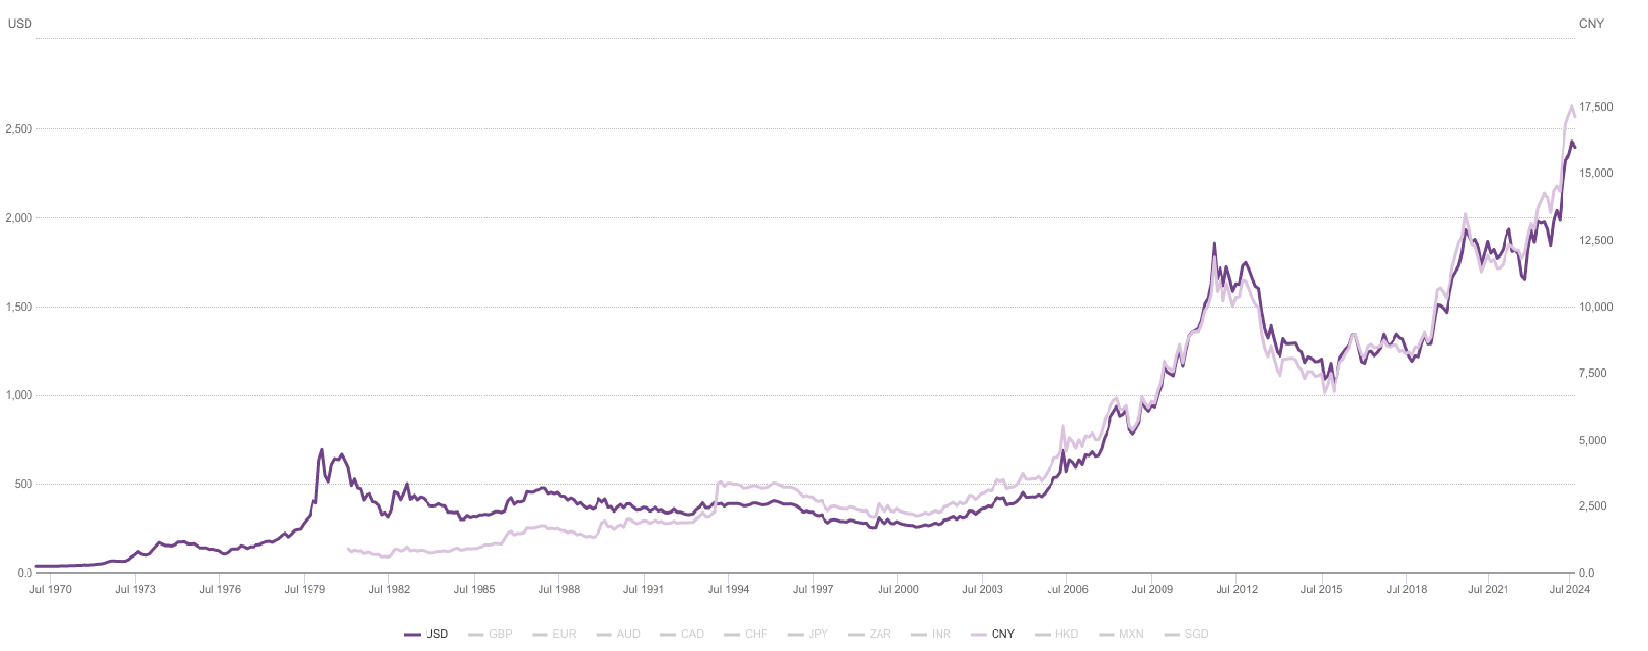
\includegraphics[width=1\linewidth]{1723066104381.png}
\end{figure}

\begin{figure}
    \centering    
    Figure 2. Total capital reserve funds in monetized-capital (U.S. current dollars) of the top-ten gold-bearers national-economies, 1960-2023
    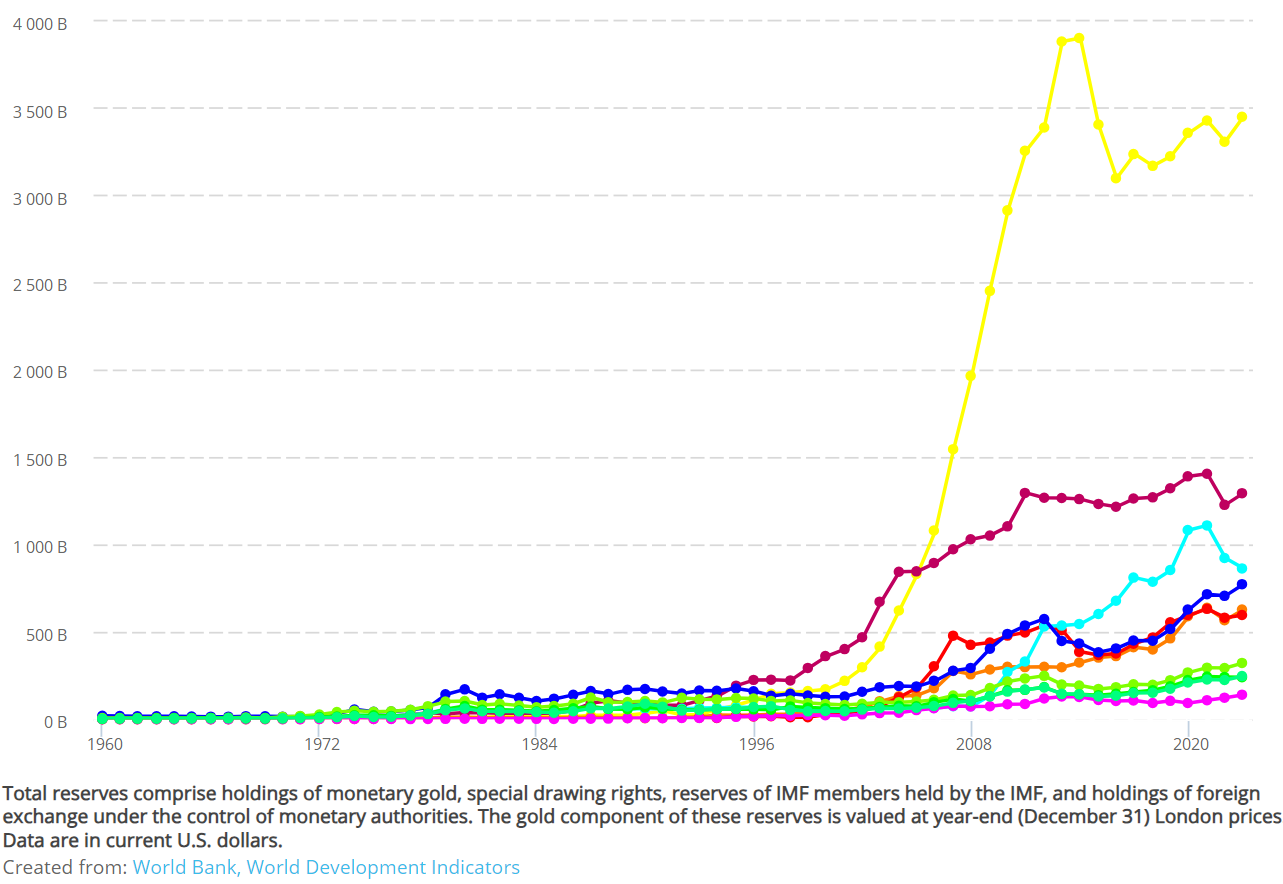
\includegraphics[width=1\linewidth]{Total reserves.PNG}
\end{figure}

\begin{figure}
    \centering   
    Figure 3. Total capital reserve funds in gold-money-capital (U.S. current dollars) of the top-ten gold-bearers national-economies, 1960-2023
    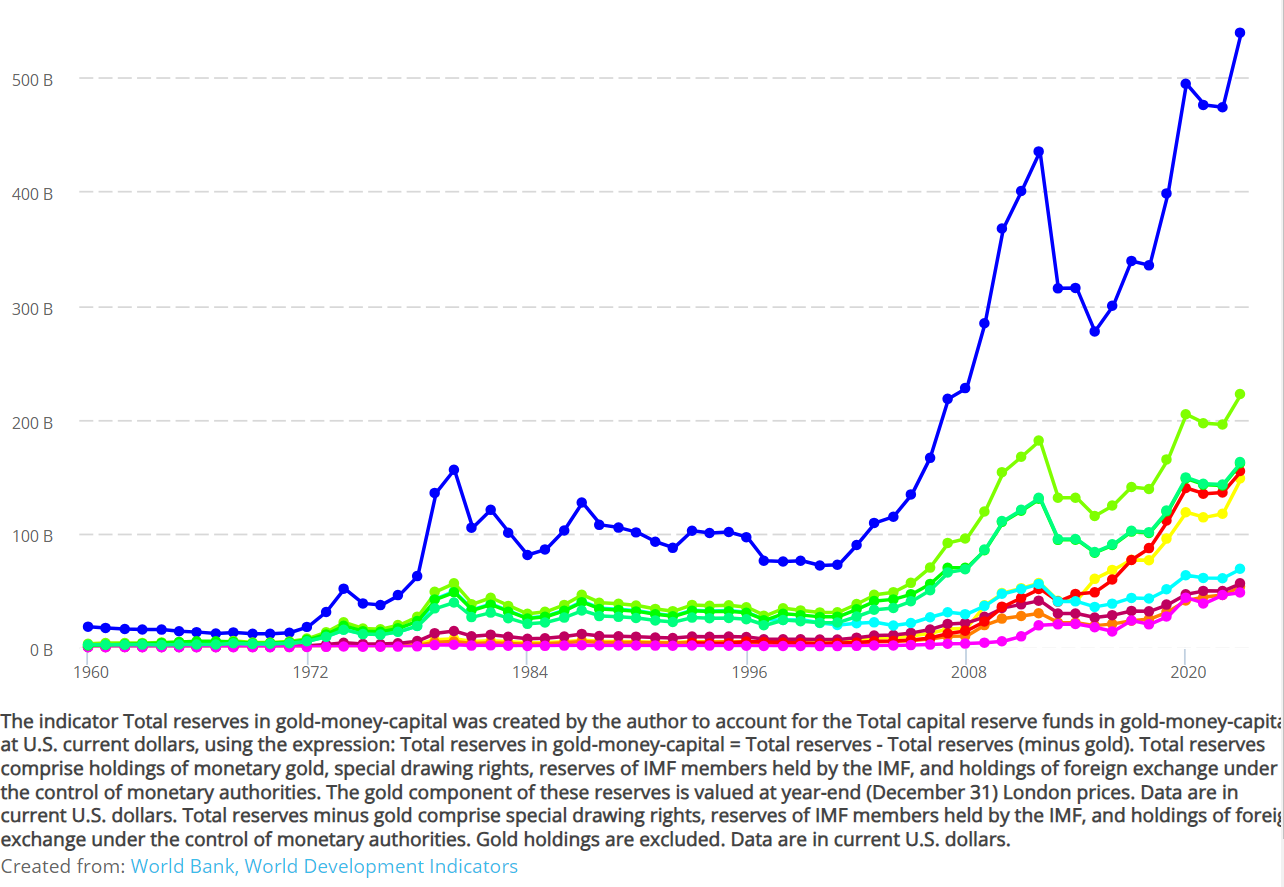
\includegraphics[width=1\linewidth]{Total gold-capital reserves.PNG}
\end{figure}

\begin{figure}
    \centering  
    Figure 4. China and U.S. total capital reserve funds in gold-money-capital (U.S. current dollars), 2000-2023
    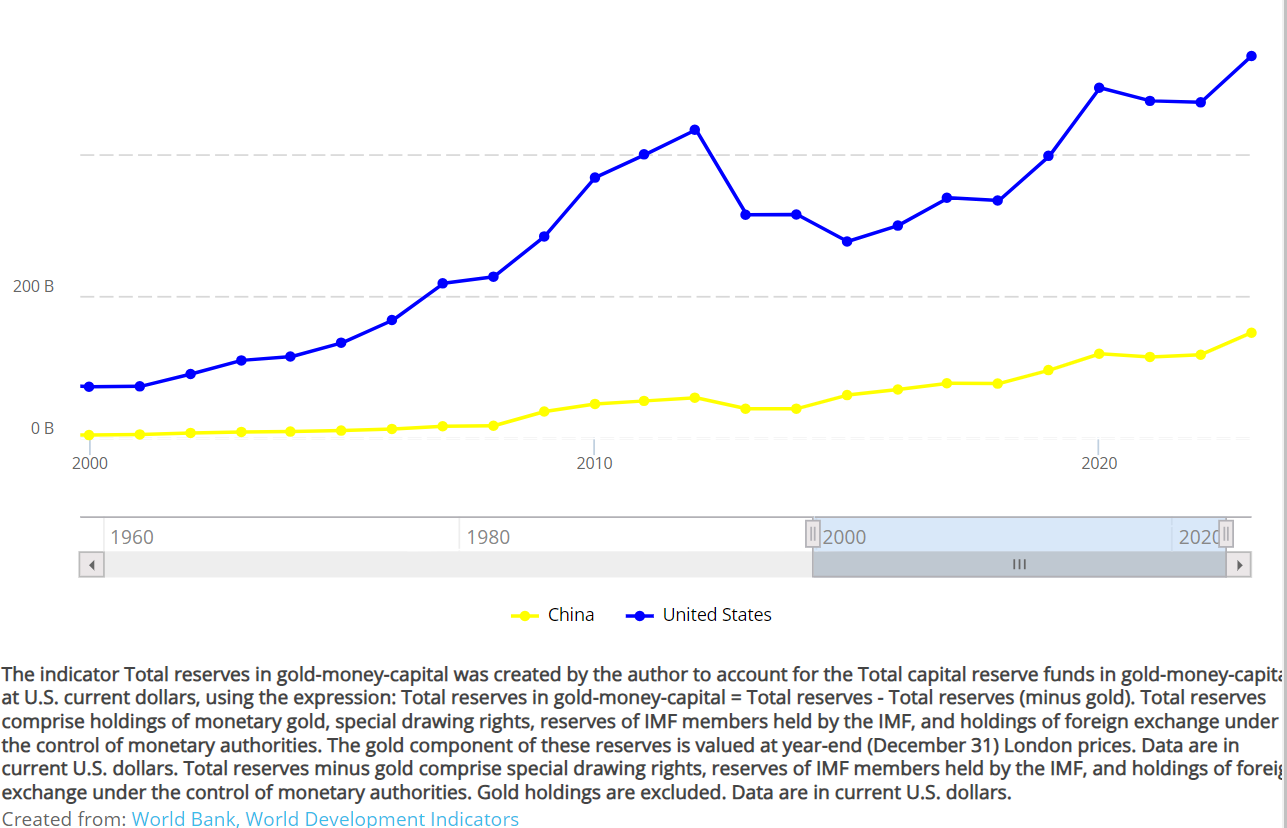
\includegraphics[width=1\linewidth]{Total gold-capital reserves-China-US.png}
\end{figure}



\end{document}